\section{Experimental Design}
\subsection{Dataset construction and audit}
The relabeled snapshot contains 418 source images: 297 Magnolia and 121 Azalea. After rejecting five zero-width rows, 29,842 usable one-class annotations remain (15,644 Magnolia; 14,198 Azalea). Three reviewed Azalea images contain no instances and are retained as source-level negatives; one unlabeled Azalea RGB frame is excluded. Magnolia images are $5184\!\times\!3888$ and Azalea images are $5280\!\times\!3956$. With $s=1024$, $\alpha=.25$, and a minimum retained-box visibility of $.5$, preprocessing yields 14,630 tiles and 1,328 boundary-aware hard negatives.

\begin{table}[t]
\centering
\wacvtablefont
\caption{Relabeled corpus and source-safe tiling snapshot. Box statistics precede tiling.}
\label{tab:data}
\setlength{\tabcolsep}{5pt}
\begin{tabular}{lrrr}
\toprule
Crop & Sources & Boxes & Tiles \\
\midrule
Magnolia & 297 & 15,644 & 10,395 \\
Azalea & 121 & 14,198 & 4,235 \\
\midrule
Total & 418 & 29,842 & 14,630 \\
\bottomrule
\end{tabular}
\end{table}

A balanced human audit samples crop, source, box-size stratum, image boundary, and annotation-density stratum. Final detector and VLM results are released only after the audit size, agreement, and exclusion rules are frozen.

\subsection{Observed cross-crop shift}
Figure~\ref{fig:domainshift} describes the transfer setting before model fitting. Azalea contains a median of 97 boxes per image versus 57 for Magnolia, while its median normalized box area is $44.1\%$ smaller. Appearance and green-fraction marginals also differ. These statistics motivate crop-disjoint evaluation; they are not presented as a causal explanation of transfer error.

\begin{figure*}[t]
    \centering
    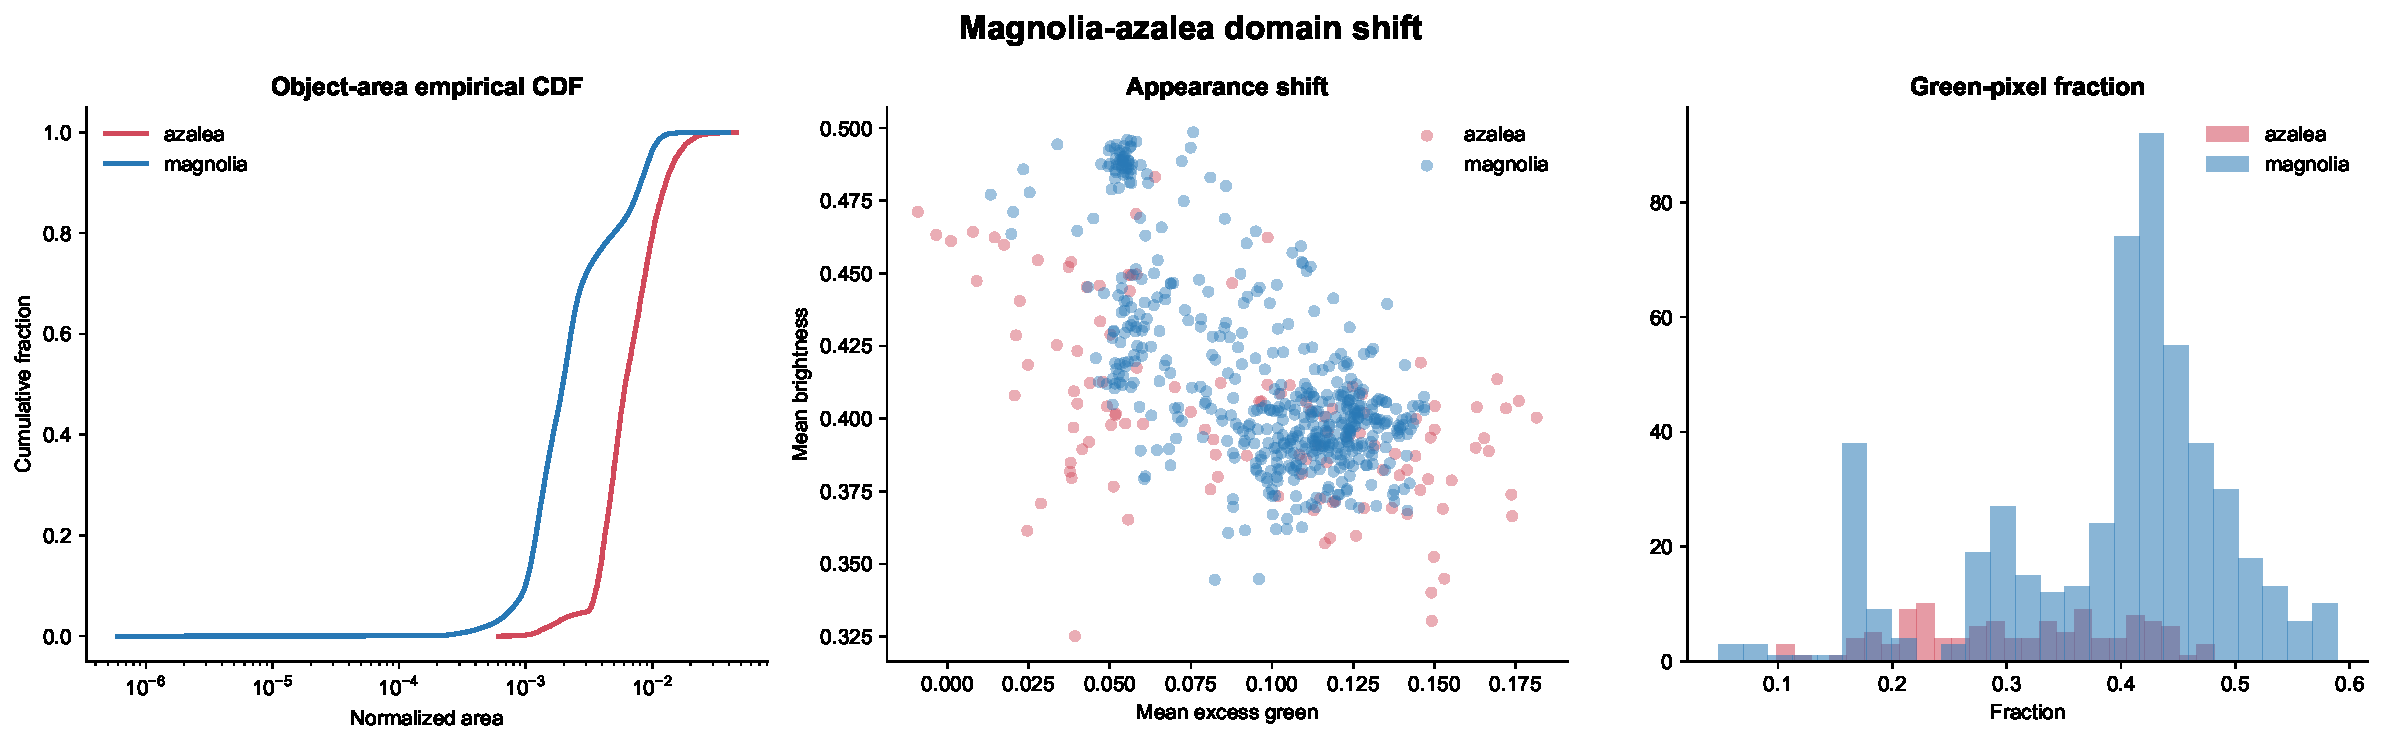
\includegraphics[width=\textwidth]{figures/cross_crop_shift.pdf}
    \caption{\textbf{Measured Magnolia--Azalea domain shift.} The object-area CDF uses valid ground-truth boxes; appearance statistics are computed once per source image. The differences in scale, density, and RGB appearance motivate directed cross-crop evaluation. No prediction is used in this figure.}
    \label{fig:domainshift}
\end{figure*}

\subsection{Source-safe evaluation protocols}
The fixed source split contains 302 training, 58 validation, and 58 test images, yielding 10,570, 2,030, and 2,030 tiles. We report five protocols: Magnolia$\rightarrow$Magnolia (M$\rightarrow$M), Azalea$\rightarrow$Azalea (A$\rightarrow$A), M$\rightarrow$A, A$\rightarrow$M, and crop-stratified pooled training. Target-crop test labels are used only for final scoring. Prompts, count bins, selector parameters, gate fitting, and checkpoint choice are frozen without test feedback.

\subsection{Models, task, and controlled baselines}
The model ladder comprises SmolVLM2-500M, SmolVLM2-2.2B, Phi-3.5-Vision, and LLaVA-1.5-7B. All models receive identical selected tiles, task schema, maximum generation length, and decoding settings. This is a model-generality study, not a claim that all four models have equal deployment cost.

Selector baselines are evaluated at the same $K$: random sampling, spatially uniform sampling, confidence-only top-$K$, count-only top-$K$, combined-score top-$K$ ($\rho=0$), and the full exploit--explore selector. Shuffled detector scores provide a negative control, while ground-truth-oracle routing is shown only as a diagnostic upper bound. Gate baselines are raw VLM confidence, schema-only rejection, the fixed weighted score in Eq.~\eqref{eq:fixedgate}, and the validation-fitted gate.

\paragraph{Detector training.}
The baseline and mined-negative variants use the same detector architecture, source split, image size, optimization schedule, augmentation policy, and validation protocol. Mining is confined to the training partition: predictions generated at confidence $.30$ are treated as unmatched when their maximum intersection over union with a training annotation is below $.30$. Candidate $1024\!\times\!1024$ crops containing any labeled plant are discarded, leaving 70 empty-label negatives for one retraining round. Checkpoint and threshold choices use validation data only, and the held-out test partition remains untouched. The separate held-out count output is not reported in this ablation because a matched baseline count run under the same post-processing configuration is unavailable.

\subsection{Metrics and statistical protocol}
Task performance is macro-F1 for presence, count bin, density, and coverage. Reliability is measured by exact schema-valid rate, hard-negative hallucination rate, false-accept rate, accepted risk at fixed coverage, coverage at a predeclared risk target, and area under the risk--coverage curve (AURC). For $N$ test records sorted by increasing predicted risk, $e_{(j)}\in\{0,1\}$ denotes whether the complete four-field task record is incorrect. We compute
\begin{equation}
R_m=\frac{1}{m}\sum_{j=1}^{m}e_{(j)},\qquad
\mathrm{AURC}=\frac{1}{N}\sum_{m=1}^{N}R_m.
\label{eq:aurc}
\end{equation}
Efficiency includes mean and p95 latency, peak resident memory, throughput, and VLM calls per source image. One unmeasured warm-up generation is performed before timing; the generation seed is deterministically derived from the frozen study seed, tile identifier, and repeat index.

All confidence intervals use 1,000 source-image cluster-bootstrap resamples. Tiles from a source image are resampled together. Model comparisons use paired bootstrap differences when the test sources coincide. Latency and memory are measured with the same hardware, software revision, precision, image resolution, warm-up, and generation length; model-loading memory is reported separately from incremental inference memory.

\subsection{Causal ablation plan}
The ablations mirror the method decomposition rather than varying unrelated settings:
\begin{enumerate}[leftmargin=*,nosep]
    \item \textbf{Ranking evidence:} confidence only, clipped count only, and their combination.
    \item \textbf{Allocation policy:} random, spatially uniform, pure top-$K$, and exploit--explore at fixed $K$.
    \item \textbf{Budget sensitivity:} $K\in\{1,2,4,8,16\}$ and $\rho\in\{0,.125,.25,.50,.75,1\}$.
    \item \textbf{Reliability evidence:} add schema validity, repeat consistency, detector agreement, and the validation-fitted gate sequentially.
    \item \textbf{Model generality:} repeat the frozen selector and gate protocol across all four VLMs.
\end{enumerate}
Tile size $s\in\{512,768,1024,1536\}$, overlap $\alpha\in\{0,.125,.25,.50\}$, prompt sensitivity, and one-versus-three-generation studies are reported in the supplement. Selector diagnostics use Eqs.~\eqref{eq:evidence-recall}--\eqref{eq:redundancy} at source-image level. Stochastic policies are repeated ten times and then averaged per source; 95\% intervals use 1,000 source-cluster bootstrap resamples.
